\documentclass{article}

%----------------------------------------------------------------------------------------
%	PACKAGES AND OTHER DOCUMENT CONFIGURATIONS
%----------------------------------------------------------------------------------------

\usepackage[T1]{fontenc}
\usepackage[utf8]{inputenc}
\usepackage{lmodern}
\usepackage[english]{babel}
\usepackage[autostyle]{csquotes}
\usepackage{graphicx} % Required for inserting images
\usepackage[hyphens]{url}
\usepackage{hyperref}
\usepackage{amsmath}      % for additional mathematical features
\usepackage{amsfonts}     % for mathbb command
\usepackage{float}
\usepackage{setspace}
\usepackage{listings}
\doublespacing
\usepackage[backend=biber,style=authoryear]{biblatex}
\renewcommand*{\bibfont}{\small}
\addbibresource{Bibliographie.bib}
\usepackage{tcolorbox}

%----------------------------------------------------------------------------------------
%	DOCUMENT MARGINS
%----------------------------------------------------------------------------------------

\usepackage{geometry} % Required for adjusting page dimensions and margins

\geometry{
	paper=a4paper, % Paper size, change to letterpaper for US letter size
	top=3cm, % Top margin
	bottom=3cm, % Bottom margin
	left=3cm, % Left margin
	right=3cm, % Right margin
	headheight = 10pt, % Header height
	footskip = 1.5cm, % Space from the bottom margin to the baseline of the footer
	headsep = 1.2cm, % Space from the top margin to the baseline of the header
	%showframe, % Uncomment to show how the type block is set on the page
}

\title{Draft}
\author{Clementine de Montgolfier}
\date{Oct/Nov 2023}

\begin{document}

\maketitle

\section{Summary, and notes for future me}

Defining optimal forest management strategies in a changing world is a challenge in the field of forest ecology. The complexity of forest ecosystems, coupled with the uncertainty of future climate conditions, makes it difficult to determine the best course of action. The concept of forest diversity is a key consideration in this debate, as it is believed to be a significant factor in the resilience of forest ecosystems. This study aims to explore whether diversity can be used as a management tool to maintain ecosystem services. To this end, we will use a theoretical model of a mixed-species, multi-layered forest, and apply control theory and viability analyses to assess the relationship between diversity and management trajectories, considering both species and vertical diversity at the stand level.\\

\noindent \textbf{Keywords:} forest management, diversity, control theory, viability theory

\section{Intro}
Eventuellement : calcul de diversité en foret, avantage attendu des différentes pratique de gestion

Defining optimal forest management strategies in a changing world is a challenge in the field of forest ecology. The complexity of forest ecosystems, coupled with the uncertainty of future climate conditions, makes it difficult to determine the best course of action. 
But forest health is already decreasing in France (REF) and to cope with the collapse of ecosystem new management practices have already been studied : replacing monospecific forets stand by mixted species stand or uneven forest management by replacing clear-cutting by retention forestry and selection cutting.\\
Knowledge on this two practices is still limited and the results are not always consensual but they are already implemented and rely on the idea that diversification is a way to increase multiple ecosystem services.\\
Work on composition diversification and its effects is mainly driven by the first work on biodiversity ecosystem functioning (BEF) from grassland studies in the 70's ~\autocite{tilmanBiodiversityPopulationEcosystem1996}.They showed that there was a positive link between biodiversity and ecosystem functioning. But the mechanisms behind this link are still not well understood. Numerous hypothesis were made to explain this link: competitive exclusion, niche complementary, sampling effect, etc. ~\autocite{aliBiodiversityEcosystemFunctioning2023}. This uncertainty makes it difficult to predict the impact of biodiversity loss, and even more in other ecosystems than grasslands.
While the hypothesis of BEF relationship, and its relevance is still debated, it fuels an entire segment of research.
The study of BEF in forest is more recent and mainly focused on the link between species diversity and productivity. A positive relattionship has been demonstrated at a global scale ~\autocite{liangPositiveBiodiversityproductivityRelationship2016}, but also in specific forest ~\autocite{morinTreeSpeciesRichness2011,paquetteEffectBiodiversityTree2011,jourdanManagingMixedStands2021}. But as for grassland the mechanisms are not understood and the interaction is not positive in every forest type. ~\autocite{forresterReviewProcessesDiversity2016}.
However one of the way to explain the contrasting results could be that the biodiversity-productivity interaction is context dependant. The relationship seems to be mostly positive in harsh climate and low tree density but negative in suitable environment ~\autocite{juckerClimateModulatesEffects2016}.
It is also reductive to consider productivity as the only characteristic of forest ecosystems, and many other should be accounted for : support of habitat and biodiversity, regulation of flood, carbon storage and also cultural and aesthetic values.
All of them might not be impacted in the same way. For example there doesn't seem to be an effect of mixture on other soil biodiversity ~\autocite{korboulewskyHowTreeDiversity2016}.
To have a better understanding of the impact of biodiversity on forest functioning it seems necessary to study multiple functions at the same time. It has been shown that diversity can increase multi-functionality by the jack-of-all-trades mechanism ~\autocite{vanderplasJackofalltradesEffectsDrive2016} while not optimizing any of them. This compromise can be seen in the balance between young and old grown forests, if the firsts are more productive, they store less carbon than the last ~\autocite{caspersenSuccessionalDiversityForest2001}. It is thus important to define the functions that we want to preserve as well as threshold for each of them.

Vertical diversity brought back in forest by uneven forest management have also been advocated to be a possible solution to the increasing fralgility of this ecosystem ~\autocite{guldinRoleUnevenAgedSilviculture1996}. Today only 25\% of managed forest in europe is composed of uneven aged stand (foresteurope.org), but the actual effect of such management is hardly consensual. In his review in 2017 Nolet ~\autocite{noletComparingEffectsEven2018} concludes that "overall, the complexity	of comparing even- and uneven- aged silviculture may explain the surprisingly limited number of studies that compare ecological effects of even- and uneven- aged silviculture".

All of this aims at increasing the diversity in forest, both in term of species and vertical structure. But the reults are not unanimous and it is impossible to extract an optimal management trajectory with our knowledge and the added complexity of maximizing multiple functions at the same time.

\subsection{Control theory and viability and utility for the subject}

There doesn't seem to be any optimal solution to manage such complicated ecosystems, while taking into account their multi-functionality. Viability theory could be an appropriate tool to define management trajectories that could keep the system in a desirable state. These desirable states have to be defined beforehand, but a lot less hypothesis and knowledge are needed for control, this allows to try different and new trajectories. This analyses define the set of desirable states that can be kept inside our constraints : the "viability kernel" \autocite{rougeExtendingViabilityTheory2013} : 
\begin{equation}
    Viab(K) = \{x_0 \in K \mid \forall t \geq 0, \exists u(\cdot), \forall t \geq 0, x(t) \in K\}
\end{equation}

This type of analyses has already be used in forest management strategy ~\autocite{mathiasUsingViabilityTheory2015}.

\subsection{Questions, objectives and hypotheses}

With this tool we want to change the question and not only ask ourselves how to increase diversity for wood productioin but can diversoty be used as a management tool to maintain ecosystem services.\\
Could we change the paradigm of forest management by using diversity as a management tool, and not simply as a side goal ?\\
What are the effect of managing composition and vertical diversity on other ecosystem services ?\\
Is it possible to define a set of management strategies that could keep the system in a desirable state ?\\

\section{Methods}

\subsection{Very short history on forest models}

Forest models are very diverse, they evolved with need, understanding of ecosystem processes, and technological innovations. They are applied at different spacial scales from tree, to stand to landscape level. They integrate different processes as growth, regeneration, mortality, management, photosynthesis, evapotranspiration, disturbances with more or less details. Numerous types of forest model classification exist ~\autocite{porteModellingMixedForest2002}, but for this short exploration only a simple classification in two groups will be useful ~\autocite{fontesModelsSupportingForest2011} : first there are the empirical models that are developed on experimental data (and then theoretical models which are the continuous equivalent with differential equation), secondly there are the process based models (PBM) that infer dynamics from underlying processes at community,individual or cellular level. Amongst PBM, the biggest family is formed by Gap-models ~\autocite{bugmannREVIEWFORESTGAP2001}, built upon the assumption that most of forest dynamic is the result of competition for light.
Although gap models show promise, a significant drawback is their complexity, especially when defining the system state. This complexity surpasses our capacity for analysis. However, it is possible to reduce dimensions (and runtime to 5\%) while making minimal assumptions with model aggregation, achieved through tools like DisCForM and TreeMig \autocite{lischkeAggregationIndividualTrees1998,lischkeTreeMigForestlandscapeModel2006} by height discretization.
Actually model aggregated by size class are close to theoretical sized structured population models. ~\autocite{bugmannREVIEWFORESTGAP2001}
On the other hand theoretical models are derived from theoretical considerations, and not from detailed mathematical models of tree population dynamics such as gap models. However both of this approach show a remarkable congruence in their formulation \autocite{bugmannREVIEWFORESTGAP2001}.
For this study the needs for stand-level mixed-species size structured forest with a limited number of state variables and the possibility to apply management strategies, led us to the choice of a theoretical model. The model is based on the work of Kohyama and associates ~\autocite{kohyamaStratificationTheoryPlant2009, kohyamaOnesidedCompetitionLight2012}.

\subsection{Our model}

Our choice of model was highly constrained by the computational memory and capacity needed by a viability analyses. The model had to be simple enough to be sumarized by a small number of state variables, but also complex enough to be able to test different management strategies.For this purpouse theorical models are a good compromise.\\

The theoretical model described below comes from the study of multiple articles from Kohyama and associates ~\autocite{kohyamaStratificationTheoryPlant2009, kohyamaOnesidedCompetitionLight2012}.
It is a compartment based model with multi species and multi layers structure Figure ~\ref{fig:fig_model}. The dynamic is influenced by growth, regeneration, mortality as well as competition processes. There are some differences between the models present in Kohyama 2009 and 2012, in particular definition of birth and competition. We chose to define birth as in Kohyama 2009 as a negative linear, or Verhulst function (and not as a negative exponential, or Ricker function in Koyama 2012). The only difference is that birth in our study is concidere on independant from the number of adult tree. This is the same hypothesis as in the gap-model ForCEEPS ~\autocite{morinUsingForestGap2020} with which we want to parameterize our model. Even if Kohyama 2009 propose a way to add competition for resources by layers below, we chose a strictly one-sided competition from the above layers as in Kohyama 2012.

\begin{figure}[h]
    \centering
    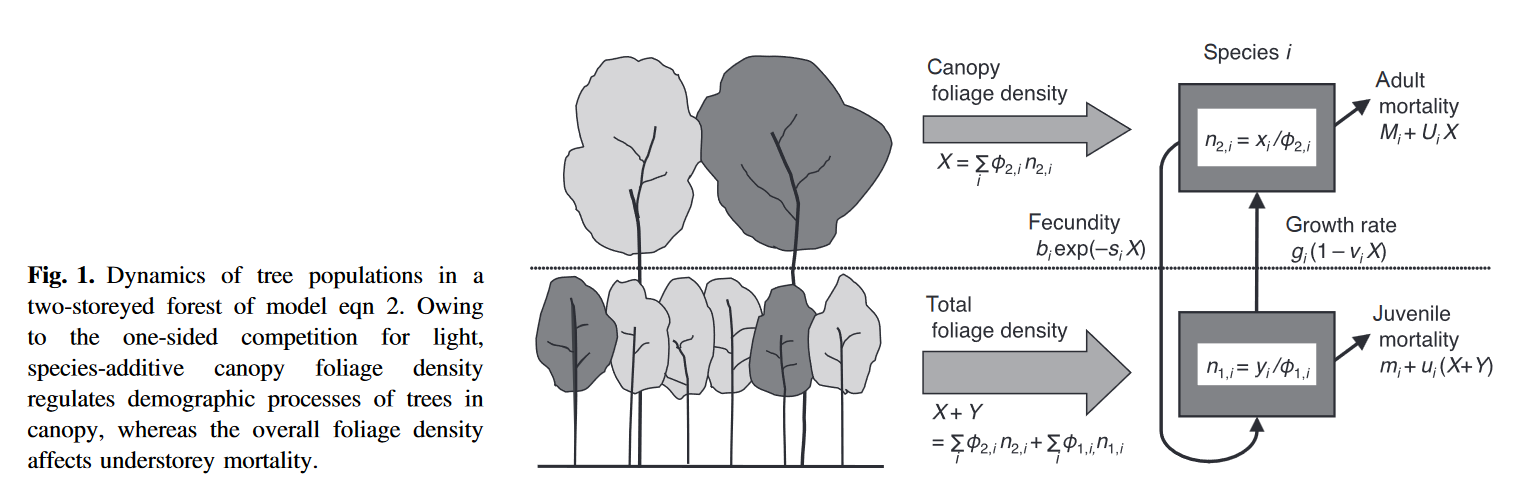
\includegraphics[width=\textwidth]{Figure/Fig_model_Kohyama.png}
    \caption{Figure from ~\autocite{kohyamaOnesidedCompetitionLight2012}}
    \label{fig:fig_model}
\end{figure}

Dynamic of each layer is driven by the competition from above layers foliage density (assimilated to the basal area) $\sum_{i = l}^{L} X_i$ with $X_i$ being the foliage density of layer $i$ :
\begin{equation}
    X_{l} = \sum_{sp} x_{sp,l} = \sum_{sp} \phi_{sp,l} n_{sp,l}
\end{equation}

The various processes are influenced by competition, with a linear negative relationship. When it comes to the birth process, optimal probabilities are determined for the processes ($b$, $g$, $m$) without competition. These probabilities are then adjusted based on the sensitivity ($Cb$, $Cg$, $Cm$) of the layer and species to foliage density.

\noindent The model can be summarised with one differential equation : \\
\begin{equation}\label{eq:model_general}
    \begin{split}
    \frac{dn_{sp,l}}{dt} = & 
    + b_{sp,l} (1 - Cb_{sp,l} \sum_{i = 1}^{L} X_{i}) \\
    & + g_{sp,l - 1} n_{sp,l-1} (1 - Cg_{sp,l-1} \sum_{i = l-1}^{L} X_{i}) \\
    & - g_{sp,l} n_{sp,l} (1 - Cg_{sp,l} \sum_{i = l}^{L} X_{i}) \\
    & - m_{sp,l} n_{sp,l}(1 + Cm_{sp,l} \sum_{i = l}^{L} X_{i})
    \end{split}
\end{equation}
\\
And some special cases for lower and upper layers : \\
\begin{center}
    $b_{sp,l} = 0$ for l > 1 \\
    $g_{sp,L} = 0$ \\
    $g_{sp,0} = 0$
\end{center}

Population densities and demographic parameters are defined in ~\ref{tab:coef} and are all positive.

\begin{table}[H]
    \centering
    \begin{tabular}{l l l}
    \hline
    \hline
    \textbf{Abbreviation} & \textbf{Meaning} & \textbf{Unit} \\
    \hline
    \hline
    $l$            & layer index                                                 &          \\
    $L$            & number of layer (i.e. maximum layer)                        &          \\
    $sp$           & species index                                               &          \\
    $SP$           & number of species                                           &            \\
    $n_{sp,l}$     & number of trees of species $sp$ in layer $l$                & $ha^{-1}$  \\    
    $x_{sp,l}$     & foliage density of species $sp$ in layer $l$                & $m^2.ha^{-1}$  \\
    $\phi_{sp,l}$     & mean basal area of tree from species $sp$ in layer $l$    & $m^2$  \\
    $X_{l}$        & foliage density of layer $l$                                & $m^2.ha^{-1}$  \\ 
    $\sum_{i = l}^{L} X_{i}$     & foliage density above layer $l$      & $m^2.ha^{-1}$  \\ 
    $b_{sp}$       & optimal birth rate per tree in layer $L$    &  \\
    $Cb_{sp}$      & birth susceptibility to superior foliage density    & $ha.m^{-2}$           \\
    $g_{sp,l}$     & growth susceptibility to superior foliage density           &  \\
    $m_{sp,l}$     & probability of intrinsic mortality           & \\
    $Cg_{sp,l}$    & growth susceptibility to superior foliage density            &   $ha.m^{-2}$  \\
    $Cb_{sp,l}$    & mortality susceptibility to superior foliage density            & $ha.m^{-2}$    \\
    \hline
    \hline
    \end{tabular}
    \caption{Parameters for the model}
    \label{tab:coef}
\end{table}

\subsection{Model parametrisation}

We are starting with a 3 layers 3 species system with a mixture of possible species oak, beech, pine, epicea, hetre, and 3 layers of dbh (cm) interval [0,27.5], [27.5,67.5], [67.5+[. We have to define all parameters in Table \ref{tab:coeftoparam}.

\begin{table}[H]
    \centering
    \begin{tabular}{l l l}
    \hline
    \hline
    \multicolumn{3}{l}{\textbf{By species}, $sp$} \\
    \hline
    $b_{sp,1}$     & optimal birth probability per tree in layer $L$ & $year^{-1}$ \\
    $Cb_{sp,1}$    & birth susceptibility to superior foliage density& \\
    \\
    \multicolumn{3}{l}{\textbf{By species $sp$ and layer $l$}} \\
    \hline
    $\phi_{sp,l}$  & foliage density per tree of species $sp$ in layer $l$  & $ha^{-1}$  \\
    $m_{sp,l}$     & probability of intrinsic mortality                     & $ha^{-1}.year^{-1}$ \\  
    $g_{sp,l}$     & optimal probability of transition from layer $l$ to the next   & $.year^{-1}$ \\
    $Cg_{sp,l}$    & growth susceptibility to superior foliage density      &            \\
    $Cm_{sp,l}$    & mortality susceptibility to superior foliage density   &            \\
    \hline
    \hline
    \end{tabular}
    \caption{Parameters that we have to define numerically}
    \label{tab:coeftoparam}
\end{table}

FORCEEPS simulations where used to adjust the dynamic of the system. 5 species where chosen to do so : Quercus petraea, Fagus sylvatica, Pinus sylvestris, Picea abies, and Abies alba. We chose a constant climate for 300 years drawn randomly from meteorologic data from Bern between 1950 and 2000 (resulting climate can be found in Fig. Appendix). We used 2 initial states. Parameters of the system were adjusted on the resulting dynamics.\\

\section{Model dynamic, equilibrium and sensitivity analyses}

\section{Control theory and viability : generality}

The viability theory provides a framework for the strategic management of dynamic systems, exemplified here through the ecological context of a forest. In this paradigm, multiple constraints on socio-ecological characteristics of the forest are chosen to define a set of desired states denoted as \(K\). All states in \(K\) meet the constraints.

The emphasis lies in determining effective management strategies that perpetually sustain the system within the state constraint set \(K\). Mathematically, this is articulated as a controlled discrete-time dynamical system:

\[
n(t+1) = g(n(t), u(t)),
\]

where \(x(t)\) signifies the system state at time \(t\), \(K\) is the set of desired states, and \(u(t) \in U\) represents the controls, with \(U\) being the set of all feasible controls.

Viability theory strives to identify all states within \(K\) for which controlled dynamics can consistently uphold the system's defining attributes. Management strategies, encapsulated by functions \(u(t)\), are instrumental in achieving this objective. Departing from the pursuit of a singular optimal state, the emphasis is on managing within a spectrum of acceptable outcomes, mitigating irreversible negative impacts.

The resultant set encompassing all states for which a management strategy exists to perpetually confine the system within the set of desirable states is termed the viability kernel (\(Viab(K)\)). Formally, this can be expressed as:

\[
Viab(K) = \{n_0 \in K \mid \forall t \geq 0, \exists u(\cdot), \forall t \geq 0, n(t) \in K\},
\]

where \(n_0\) denotes the initial state of the system. Within the viability kernel, the system maintains a state deemed desirable.

After the delimitation of the viability kernel all viable controls (\(u_v\)) can be determined and analysed.

an algorithm inspired by Saint-Pierre (1994) is employed, accompanied by Euler integration with a 1-year timestep for temporal discretization.

\section{Control theory and viability : study case}
What is our control, the constraints we want to define

\section{Discussion}

Landscape diversity

\subsection{Forest diversity, may be more complex than diversity drives diversity}

In forests diversity can be define in different ways : Composition or structural diversity. And at different scale from the stand to the landscape.\\
Work on composition diversification and its effects is mainly driven by the first work on biodiversity ecosystem functioning (BEF) from grassland studies in the 70's ~\autocite{tilmanBiodiversityPopulationEcosystem1996}.They showed that there was a positive link between biodiversity and ecosystem functioning. But the mechanisms behind this link are still not well understood. Numerous hypothesis were made to explain this link: competitive exclusion, niche complementary, sampling effect, etc. ~\autocite{aliBiodiversityEcosystemFunctioning2023}. This uncertainty makes it difficult to predict the impact of biodiversity loss, and even more in other ecosystems than grasslands.
While the hypothesis of BEF relationship, and its relevance is still debated, it fuels an entire segment of research.
The study of BEF in forest is more recent and mainly focused on the link between species diversity and productivity. A positive relattionship has been demonstrated at a global scale ~\autocite{liangPositiveBiodiversityproductivityRelationship2016}, but also in specific forest ~\autocite{morinTreeSpeciesRichness2011,paquetteEffectBiodiversityTree2011,jourdanManagingMixedStands2021}. But as for grassland the mechanisms are not understood and the interaction is not positive in every forest type. ~\autocite{forresterReviewProcessesDiversity2016}.
However one of the way to explain the contrasting results could be that the biodiversity-productivity interaction is context dependant. The relationship seems to be mostly positive in harsh climate and low tree density but negative in suitable environment ~\autocite{juckerClimateModulatesEffects2016}.
It is also reductive to consider productivity as the only characteristic of forest ecosystems, and many other should be accounted for : support of habitat and biodiversity, regulation of flood, carbon storage and also cultural and aesthetic values.
All of them might not be impacted in the same way. For example there doesn't seem to be an effect of mixture on other soil biodiversity ~\autocite{korboulewskyHowTreeDiversity2016}.
To have a better understanding of the impact of biodiversity on forest functioning it seems necessary to study multiple functions at the same time. It has been shown that diversity can increase multi-functionality by the jack-of-all-trades mechanism ~\autocite{vanderplasJackofalltradesEffectsDrive2016} while not optimizing any of them. This compromise can be seen in the balance between young and old grown forests, if the firsts are more productive, they store less carbon than the last ~\autocite{caspersenSuccessionalDiversityForest2001}. It is thus important to define the functions that we want to preserve as well as threshold for each of them.

Actually species diversity is not the only way to bring back diversity in forest and recently vertical diversity in forest have also been advocated to be a possible solution to the increasing fralgility of this ecosystem ~\autocite{guldinRoleUnevenAgedSilviculture1996}. Today only 25\% of managed forest in europe is composed of uneven aged stand (foresteurope.org), but the actual effect of such management is hardly consensual. In his review in 2017 Nolet ~\autocite{noletComparingEffectsEven2018} concludes that "overall, the complexity	of comparing even- and uneven- aged silviculture may explain the surprisingly limited number of studies that compare ecological effects of even- and uneven- aged silviculture".

\subsection{Management for diversity}

Forest management is inextricably linked to the evolving understanding of ecological dynamics and global shifts. In addressing the question of how to manage diversity in managed forests, several propositions or practice philosophies have been put forth. The first is avoiding clear-cutting which can be done in a number of ways. First retention forestry \autocite{gustafssonRetentionForestryMaintain2012,rosenvaldWhatWhenWhere2008} aims at maintaining the structure and composition of the forest by leaving a certain proportion of trees in the stand after harvesting. This approach is based on the assumption that the forest will regenerate naturally, and that the retained trees will provide a seed source for the next generation, it is also a way to keep a certain diversity on the stand. The second is the choice of an irregular Shelterwood Systems (also called uneven aged forest or continuous cover forestry) \autocite{sinhaOptimalManagementNaturally2017,schallImpactEvenagedUnevenaged2018,nylandEvenUnevenagedChallenges2003,noletComparingEffectsEven2018,dudumanForestManagementPlanning2011} which aims to maintain a continuous cover of trees in the stand, and some vertical diversity. The second thing to rely on mixture of species \autocite{morinTreeSpeciesRichness2011,jourdanManagingMixedStands2021}, while eventually consideration the plantation of tree species resilient to future climate conditions \autocite{websterPromotingMaintainingDiversity2018}.

The complexity of these approaches underscores the need for a comprehensive study of forest management practices to ascertain their effectiveness while mitigating drawbacks.

\printbibliography

\section{Appendix}

\subsection{Parametrization}

For parametrisation we used 
\begin{lstlisting}
optim(init_parameter, distance_model_data, ,method = "CG")
\end{lstlisting}

optim function with algorithm : 

Resulting parameters :

TABLE

\end{document}


























%%%%%%%%%%%%%%%%%%%%%%%%%%%%%%%%

some text that have been removed

%%%%%%%%%%%%%%%%%%%%%%%%%%%%%%%%

I said before, IBMs are too complex to run at large scale. A more
efficient approach would be to derive suitable mathematical equations to
scale correctly from parameters governing individual trees to the dynamics
of forested region (Kohyama et al., 2001; Hurtt et al., 1998; Moorcroft et al.,
2001; Kohyama, 2005


\subsection{Matrix transition model Buongiorno}

Matrix model parameterized for 3 species : Fir, spruce, beech in the french Jura. With a sized-structured population in 9 strata. ~\autocite{buongiornoMatrixModelUnevenAged1980}

Processes are : growth, mortality and recruitment defined as follow :
\begin{equation}
    g_{str,sp} = a_{sp} + b_{sp} BA + c_{sp} D_str
\end{equation}
\begin{equation}
    m_{str,sp} = d_{sp} + e_{sp} BA + f_{sp} D_str
\end{equation}
\begin{equation}
    r_{sp} = smthing
\end{equation}

\subsection{DisCForM}

DisCForM ~\autocite{lischkeAggregationIndividualTrees1998} is an aggregated model of the Forclim (version 2.4.0.2) gap model ~\autocite{bugmannSimplifiedForestModel1996}.

The main points of \textit{DisCForM} are:
\begin{enumerate}
    \item The continuous height distribution $(2.5)$ of the trees in a patch model is replaced by the discrete height structure
    \item The entire forest is simulated at once in each time step.
    \item The half empirical process functions and probabilities of a patch model for birth, growth, and mortality of trees are still used.
    \item The spatial distribution of trees per unit area is modeled by the assumption that in each time step all trees of a certain height are randomly distributed over the forest.
\end{enumerate}

It approximates ForClim with a 76\% similarity rate for only 4.09\% of run-time.

\begin{figure}[h]
\centering
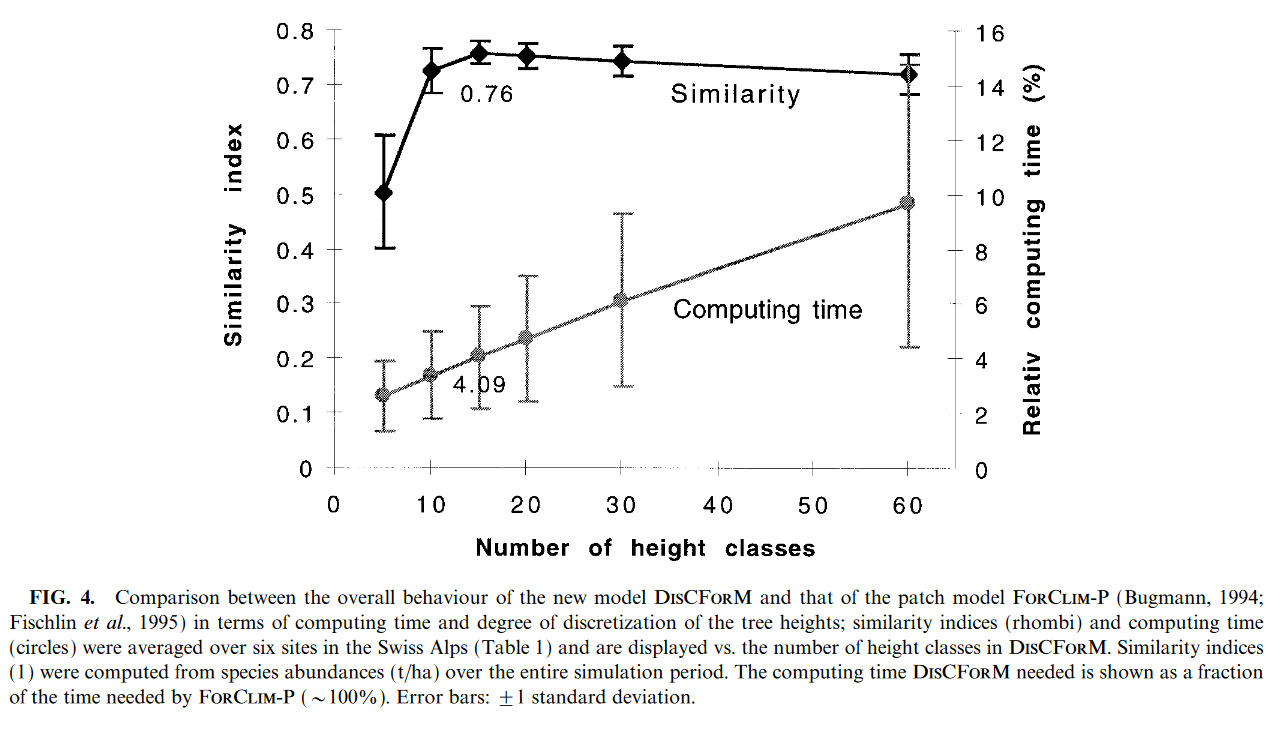
\includegraphics[width=\textwidth]{Figure/DiCForM_performances.png}
\caption{Figure from ~\autocite{lischkeAggregationIndividualTrees1998}}
\end{figure}


Considering aggregation, DISCFORM can be expressed as a system of Ordinary Differential Equations (ODEs) given by: ~\autocite{lofflerIncorporationInfluenceVariability2001}

\[
\dot{y}_{s,k} = \bar{g}_{s,k-1}y_{s,k-1} - \bar{g}_{s,k}y_{s,k} - \bar{m}_{s,k}y_{s,k} + \bar{b}_{s,k}, \quad s, k \in \mathbb{N}^*
\]

where \(y_{s,k}\) represents the mean of the population density \(N_{s,k}\) per patch area of trees of species \(s\) in height class \(k\). The rate of change of \(y_{s,k}\) at time \(t\) is influenced by mortality (\(\bar{m}_{s,k}\)), birth (\(\bar{b}_{s,k}\)), and growth (\(\bar{g}_{s,k}\)) processes. These processes operate between height classes \(k-1\) and \(k\), with trees growing into class \(k\) from class \(k-1\) and leaving by outgrowing it.

The rates \(\bar{g}_{s,k}\), \(\bar{m}_{s,k}\), and \(\bar{b}_{s,k}\) depend on the available light in a height class and are influenced by time-dependent input variables such as temperature, precipitation, and nitrogen.

Today exist in the form of Treemig ~\autocite{lischkeTreeMigForestlandscapeModel2006} which also integrate tree migration between patches thought seed dispersal. Documentation for Treemig is accessible at : \url{https://treemig.wsl.ch/en/}, and code depository for R wrapper at \url{https://gitlabext.wsl.ch/boehmd/treemig}. The scale of this model is the landscape but a study at the patch level is still possible by analysing only one cell of the landscape.

Equations
Parameters

\textbf{The limit is that it is coded for 15 layers (a lot, but also necessary to be close from reality) and in FORTRAN}

Disadvantage of aggregated models is that their derivation is based on some simplifying assumptions so that the PDE approximation may deviate from that of the gap model. Still, the value of a PDE approximation lies in its potential to perform systematic behavior analyses of the gap model with respect to both its parameter space as well as driving variables such as climate. And there is always the possibility to double check weird trajectory with the initial individual centered gap-model. 